\documentclass[12pt,a4paper,fontset=fandol]{ctexart}

\usepackage{geometry}
\geometry{left=2.6cm,right=2.6cm,top=2.6cm,bottom=2.6cm}
\usepackage{graphicx}
\usepackage{booktabs}
\usepackage{longtable}
\usepackage{array}
\usepackage{float}
\usepackage{xcolor}
\usepackage{listings}
\usepackage{caption}
\usepackage{hyperref}
\usepackage{fancyhdr}

\hypersetup{
  colorlinks=true,
  linkcolor=black,
  urlcolor=blue
}

\pagestyle{fancy}
\fancyhf{}
\fancyhead[L]{Linux 基础与 ANNOVAR FASTA 序列统计}
\fancyhead[R]{\thepage}
\renewcommand{\headrulewidth}{0.4pt}
\setlength{\headheight}{15pt}

\captionsetup{font=small,labelfont=bf}

\lstdefinestyle{linuxcode}{
  basicstyle=\ttfamily\small,
  breaklines=true,
  columns=fullflexible,
  frame=single,
  framerule=0.3pt,
  rulecolor=\color{gray!45},
  backgroundcolor=\color{gray!6},
  xleftmargin=0.5em,
  xrightmargin=0.5em,
  aboveskip=0.7em,
  belowskip=0.7em
}

\lstdefinestyle{resultcode}{
  basicstyle=\ttfamily\small,
  breaklines=true,
  columns=fullflexible,
  frame=single,
  framerule=0.3pt,
  rulecolor=\color{gray!45},
  backgroundcolor=\color{blue!3},
  xleftmargin=0.5em,
  xrightmargin=0.5em,
  aboveskip=0.7em,
  belowskip=0.7em
}

\lstdefinelanguage{R}{
  morekeywords={
    if, else, repeat, while, function, for, in, next, break,
    TRUE, FALSE, NULL, NA, NaN, Inf,
    readLines, startsWith, sub, grepl, as.data.frame, table, names,
    match, paste0, data.frame, c, merge, as.integer, order, write.csv,
    cor, sink, cat, sprintf, png, par, plot, text, lm, abline, legend, dev.off
  },
  sensitive=true,
  morecomment=[l]{\#},
  morestring=[b]",
  morestring=[b]'
}

\lstdefinestyle{rcode}{
  language=R,
  basicstyle=\ttfamily\small,
  keywordstyle=\color{blue!70!black}\bfseries,
  commentstyle=\color{green!40!black}\itshape,
  stringstyle=\color{red!55!black},
  identifierstyle=\color{black},
  numberstyle=\color{purple!70!black},
  breaklines=true,
  columns=fullflexible,
  frame=single,
  framerule=0.35pt,
  rulecolor=\color{blue!35!black},
  backgroundcolor=\color{blue!4},
  xleftmargin=0.5em,
  xrightmargin=0.5em,
  aboveskip=0.7em,
  belowskip=0.7em,
  showstringspaces=false
}

\title{\heiti Linux 基础与 ANNOVAR\\FASTA 序列统计实验报告}
\author{
学院：元培学院 \qquad 姓名：高禹宸\\
学号：2400017417 \qquad 班级：周二班
}
\date{2026 年 4 月 30 日}

\begin{document}
\maketitle
\thispagestyle{empty}

\section{实验目的}

本实验依据课程 PDF《Introduction to Linux for Biological Sciences》完成 Linux 基础操作与 ANNOVAR FASTA 文件分析。主要目标包括：

\begin{itemize}
  \item 掌握 Linux/macOS 终端中的目录创建、路径切换、文件复制、删除、解压和帮助查询；
  \item 安装并检查基因组注释工具 ANNOVAR，理解其示例目录和 FASTA 文件格式；
  \item 使用 grep、wc、重定向、Bash 脚本等工具统计特定染色体上的 RNA 序列数量；
  \item 比较所有常染色体 RNA 序列数量，并用 R 可视化其与染色体长度之间的关系；
  \item 讨论 RNA 序列数量是否与染色体长度成比例，以及可能影响这种关系的因素。
\end{itemize}

\section{背景介绍}

Linux 命令行是生物信息学实验中常用的数据处理环境。相比图形界面，命令行更适合处理大规模文本文件、批量运行程序和构建可复现分析流程。
在本实验对使用linux的练习实践示例数据中包含多个标准生物信息学文件，对于这些文件可以进行整理和分析。

FASTA 文件通常由描述行和序列行组成。描述行以 ``>'' 开头，后续为核酸或蛋白序列。本次实验分析的文件为 \texttt{hg38\_refGeneWithVerMrna.fa}，其中描述行包含 RefGene 转录本编号、染色体位置和 ANNOVAR 生成信息。通过筛选描述行中染色体位置字段，可以统计不同染色体上的 RNA 序列数量。

\section{实验材料与方法}

\subsection{实验材料}

\begin{table}[H]
\centering
\caption{实验材料与文件}
\begin{tabular}{lll}
\toprule
材料 & 文件或来源 & 用途 \\
\midrule
课程说明 & \texttt{c4.Linux\_basics.pdf} & 实验要求与得分点 \\
终端记录 & \texttt{终端保存的输出.txt} & 课堂已完成命令和结果 \\
分析软件 & \texttt{annovar.latest.tar.gz} & ANNOVAR 安装包 \\
FASTA 文件 & \texttt{hg38\_refGeneWithVerMrna.fa} & RNA 序列统计 \\
染色体长度 & GRCh38 chromosome lengths & 长度与 RNA 序列数量比较 \\
\bottomrule
\end{tabular}
\end{table}

\subsection{总体分析流程}

本实验的整体流程为：创建课程目录，复制并删除 ANNOVAR 压缩包进行文件操作练习，解压 ANNOVAR，查看 README 和 FASTA 文件，筛选 chr21 序列描述行，编写 Bash 脚本统计 chr21 和所有常染色体 RNA 序列数量，最后用 R 绘图并讨论染色体长度与 RNA 序列数量的关系。

\section{逐项实验结果}

\subsection{创建课程目录并验证当前位置}

\noindent\textbf{Linux 代码：}
\begin{lstlisting}[style=linuxcode]
cd ~
mkdir /Users/gaoyuchen/Desktop/bioinfor
cd /Users/gaoyuchen/Desktop/bioinfor
pwd
\end{lstlisting}

\noindent\textbf{实验结果：}
\begin{lstlisting}[style=resultcode]
/Users/gaoyuchen/Desktop/bioinfor
\end{lstlisting}

该结果说明课程目录创建成功，并且当前工作目录已经切换到 \texttt{bioinfor}。

\subsection{复制 ANNOVAR 压缩包并用 ls 验证}

\noindent\textbf{Linux 代码：}
\begin{lstlisting}[style=linuxcode]
cp /Users/gaoyuchen/Desktop/homework4/annovar.latest.tar.gz /Users/gaoyuchen/Desktop/bioinfor
ls /Users/gaoyuchen/Desktop/bioinfor
\end{lstlisting}

\noindent\textbf{实验结果：}
\begin{lstlisting}[style=resultcode]
annovar.latest.tar.gz
\end{lstlisting}

\texttt{ls} 输出中出现 \texttt{annovar.latest.tar.gz}，说明压缩包已复制到课程目录。

\subsection{用 bash 删除复制出的压缩包并验证}
\noindent\textbf{Linux 代码：}
\begin{lstlisting}[style=linuxcode]
rm /Users/gaoyuchen/Desktop/bioinfor/annovar.latest.tar.gz
ls /Users/gaoyuchen/Desktop/bioinfor
\end{lstlisting}

\noindent\textbf{实验结果：}
\begin{lstlisting}[style=resultcode]
# 无输出
\end{lstlisting}

删除后 \texttt{ls} 没有显示文件，说明该压缩包已从课程目录删除。

\subsection{运行并解释 tar 解压命令}
\noindent\textbf{Linux 代码：}
\begin{lstlisting}[style=linuxcode]
tar --help
tar -zxvf /Users/gaoyuchen/Desktop/bioinfor/annovar.latest.tar.gz
\end{lstlisting}

\noindent\textbf{实验结果节选：}
\begin{lstlisting}[style=resultcode]
x annovar/
x annovar/example/
x annovar/example/ex1.avinput
x annovar/example/README
x annovar/humandb/
x annovar/humandb/hg38_refGeneWithVerMrna.fa
x annovar/annotate_variation.pl
x annovar/table_annovar.pl
\end{lstlisting}

帮助来源为 \texttt{tar --help}。\texttt{-x} 表示解包，\texttt{-z} 表示通过 gzip 解压，\texttt{-v} 表示显示处理过程，\texttt{-f} 表示指定压缩包文件。终端输出显示 ANNOVAR 目录、示例文件和 humandb 数据库文件均被解压。

\subsection{用 cat 查看 ANNOVAR README}

\noindent\textbf{Linux 代码：}
\begin{lstlisting}[style=linuxcode]
cat /Users/gaoyuchen/Desktop/bioinfor/annovar/example/README
\end{lstlisting}

\noindent\textbf{实验结果节选：}
\begin{lstlisting}[style=resultcode]
visit ANNOVAR website at http://www.openbioinformatics.org/annovar for more exmaple.

ex1.avinput: a simple ANNOVAR input example with a few variants
ex2.vcf: a simple VCF file with genotype information for 3 samples
gene_xref.txt: an example gene cross-reference file
humandb/hg19_example_db_generic.txt: an example file for generic database
\end{lstlisting}

README 文件说明了 ANNOVAR 示例数据中 avinput、VCF、gene cross-reference 和示例数据库文件的用途。

\subsection{用 less 查看 FASTA 并搜索 chr22}

\noindent\textbf{Linux 代码：}
\begin{lstlisting}[style=linuxcode]
less /Users/gaoyuchen/Desktop/bioinfor/annovar/humandb/hg38_refGeneWithVerMrna.fa
# 在 less 中输入：
/chr22
# 按 n 查看下一个匹配，按 q 退出
\end{lstlisting}

\noindent\textbf{实验结果示意：}
\begin{lstlisting}[style=resultcode]
>NM_... Comment: this sequence (leftmost exon at chr22:...) is generated by ANNOVAR ...
\end{lstlisting}

通过对比可知，FASTA 文件较大，不适合一次性用 \texttt{cat} 全部输出；\texttt{less} 可以分页查看并用 \texttt{/chr22} 搜索包含 chr22 的序列描述行。

\subsection{筛选 chr21 行并导出为 hg38\_chr21.txt}

\noindent\textbf{得分点要求：} 在 FASTA 文件中筛选包含 \texttt{chr21} 的行，输出到 \texttt{hg38\_chr21.txt}，并查看新文件。

\noindent\textbf{Linux 代码：}
\begin{lstlisting}[style=linuxcode]
grep "chr21" /Users/gaoyuchen/Desktop/bioinfor/annovar/humandb/hg38_refGeneWithVerMrna.fa > hg38_chr21.txt
cat hg38_chr21.txt
mv /Users/gaoyuchen/hg38_chr21.txt /Users/gaoyuchen/Desktop/bioinfor
wc -l /Users/gaoyuchen/Desktop/bioinfor/hg38_chr21.txt
head -n 3 /Users/gaoyuchen/Desktop/bioinfor/hg38_chr21.txt
\end{lstlisting}

\noindent\textbf{实验结果：}
\begin{lstlisting}[style=resultcode]
1121 /Users/gaoyuchen/Desktop/bioinfor/hg38_chr21.txt
>NR_104257.2   Comment: this sequence (leftmost exon at chr21:41798224) ...
>NM_001001438.2 Warning: ... (leftmost exon at chr21:46188445) ...
>NM_004571.5   Comment: this sequence (leftmost exon at chr21:42974561) ...
\end{lstlisting}

输出文件 \texttt{bioinfor/hg38\_chr21.txt} 共 1121 行，说明筛选出的 chr21 相关描述行数量为 1121。

\subsection{Bash 脚本统计 chr21 序列数量}

\noindent\textbf{得分点要求：} 脚本接受一个 FASTA 格式文件作为输入，输出 chr21 上的 RNA 序列数量。

\noindent\textbf{Linux 代码：}
\begin{lstlisting}[style=linuxcode]
#!/bin/bash

file="$1"
grep -c "^>.*chr21" "$file"

chmod +x count_chr21.sh
./count_chr21.sh /Users/gaoyuchen/Desktop/bioinfor/annovar/humandb/hg38_refGeneWithVerMrna.fa
\end{lstlisting}

\noindent\textbf{实验结果：}
\begin{lstlisting}[style=resultcode]
1121
\end{lstlisting}

脚本输出 1121，与 \texttt{hg38\_chr21.txt} 的行数一致。

\subsection{在脚本中检查输入文件是否存在}

\noindent\textbf{Linux 代码：}
\begin{lstlisting}[style=linuxcode]
#!/bin/bash

file="$1"
if [ ! -f "$file" ]; then
  echo "Error: input FASTA file does not exist."
  exit 1
fi

grep -c "^>.*leftmost exon at chr21[:_]" "$file"
\end{lstlisting}

\noindent\textbf{实验结果：}
\begin{lstlisting}[style=resultcode]
# 输入正确文件时：
1121

# 输入不存在文件时：
Error: input FASTA file does not exist.
\end{lstlisting}

使用 \texttt{-f} 判断输入是否为普通文件，可以避免空参数或错误路径导致 \texttt{grep} 报错。

\subsection{循环比较所有常染色体 RNA 序列数量与 R 可视化结果}

\noindent\textbf{得分点要求：} 在上一题基础上，用循环统计 chr1 到 chr22 的 RNA 序列数量。

\noindent\textbf{Linux 代码：}
\begin{lstlisting}[style=linuxcode]
#!/bin/bash

file="$1"
if [ ! -f "$file" ]; then
  echo "Error: input FASTA file does not exist."
  exit 1
fi

for i in {1..22}; do
  chr="chr${i}"
  count=$(grep -c "^>.*leftmost exon at ${chr}[:_]" "$file")
  printf "%s\t%s\n" "$chr" "$count"
done
\end{lstlisting}

\noindent\textbf{实验结果：}
\begin{lstlisting}[style=resultcode]
chr1    7845
chr2    5583
chr3    4943
chr4    3024
chr5    3689
chr6    6988
chr7    3989
chr8    3094
chr9    3063
chr10   3611
chr11   4869
chr12   3977
chr13   1510
chr14   2546
chr15   3002
chr16   3400
chr17   4615
chr18   1279
chr19   6909
chr20   1970
chr21   1121
chr22   1863
\end{lstlisting}

统计结果已保存为 \texttt{report/chr\_sequence\_counts\_autosomes.csv}，用于后续 R 可视化和相关性分析。

\medskip
\noindent\textbf{R 可视化与相关性分析：}

\noindent\textbf{Linux 代码：}
\begin{lstlisting}[style=linuxcode]
Rscript report/make_chr_analysis.R
\end{lstlisting}

\noindent\textbf{R 脚本内容（\texttt{make\_chr\_analysis.R}）：}

这一部分R语言脚本为vibe coding得到：

\begin{lstlisting}[style=rcode]
input <- "bioinfor/annovar/humandb/hg38_refGeneWithVerMrna.fa"

headers <- readLines(input, warn = FALSE)
headers <- headers[startsWith(headers, ">")]

chr <- sub(".*leftmost exon at (chr[0-9XY]+)[:_].*", "\\1", headers)
chr <- chr[grepl("^chr([1-9]|1[0-9]|2[0-2]|X|Y)$", chr)]

counts <- as.data.frame(table(chr), stringsAsFactors = FALSE)
names(counts) <- c("chromosome", "rna_sequence_count")
counts$chr_order <- match(counts$chromosome, c(paste0("chr", 1:22), "chrX", "chrY"))
counts <- counts[order(counts$chr_order), c("chromosome", "rna_sequence_count")]

lengths <- data.frame(
  chromosome = paste0("chr", 1:22),
  length_bp = c(
    248956422, 242193529, 198295559, 190214555, 181538259, 170805979,
    159345973, 145138636, 138394717, 133797422, 135086622, 133275309,
    114364328, 107043718, 101991189, 90338345, 83257441, 80373285,
    58617616, 64444167, 46709983, 50818468
  )
)

autosomes <- merge(counts, lengths, by = "chromosome")
autosomes$chr_num <- as.integer(sub("chr", "", autosomes$chromosome))
autosomes <- autosomes[order(autosomes$chr_num), ]
autosomes$length_mb <- autosomes$length_bp / 1e6
autosomes$rna_per_mb <- autosomes$rna_sequence_count / autosomes$length_mb
autosomes <- autosomes[, c("chromosome", "length_bp", "length_mb", "rna_sequence_count", "rna_per_mb")]

write.csv(counts, "report/chr_sequence_counts_all.csv", row.names = FALSE)
write.csv(autosomes, "report/chr_sequence_counts_autosomes.csv", row.names = FALSE)

cor_value <- cor(autosomes$length_mb, autosomes$rna_sequence_count)
sink("report/correlation_summary.txt")
cat(sprintf("Pearson correlation between autosome length and RNA sequence count: %.3f\n", cor_value))
cat(sprintf("chr21 RNA sequence count: %d\n", counts$rna_sequence_count[counts$chromosome == "chr21"]))
sink()

png("report/chr_length_vs_rna_count.png", width = 1800, height = 1200, res = 180)
par(mar = c(5, 5, 3, 1))
plot(
  autosomes$length_mb,
  autosomes$rna_sequence_count,
  pch = 19,
  col = "#2F6F73",
  xlab = "Chromosome length (Mb)",
  ylab = "RNA sequence count",
  main = "RNA sequence count vs. chromosome length (autosomes)"
)
text(
  autosomes$length_mb,
  autosomes$rna_sequence_count,
  labels = autosomes$chromosome,
  pos = 3,
  cex = 0.72,
  col = "#333333"
)
fit <- lm(rna_sequence_count ~ length_mb, data = autosomes)
abline(fit, col = "#C55A11", lwd = 2)
legend(
  "topleft",
  legend = sprintf("Pearson r = %.3f", cor_value),
  bty = "n",
  text.col = "#333333"
)
dev.off()

png("report/chr_rna_counts_barplot.png", width = 1800, height = 1000, res = 180)
par(mar = c(5, 5, 3, 1))
barplot(
  counts$rna_sequence_count,
  names.arg = counts$chromosome,
  col = "#7FA8A9",
  border = NA,
  las = 2,
  ylab = "RNA sequence count",
  main = "RNA sequence count by chromosome"
)
dev.off()
\end{lstlisting}

\noindent\textbf{实验结果：}
\begin{lstlisting}[style=resultcode]
生成文件：
report/chr_rna_counts_barplot.png
report/chr_length_vs_rna_count.png
report/chr_sequence_counts_all.csv
report/chr_sequence_counts_autosomes.csv
report/correlation_summary.txt
\end{lstlisting}

\begin{figure}[H]
\centering
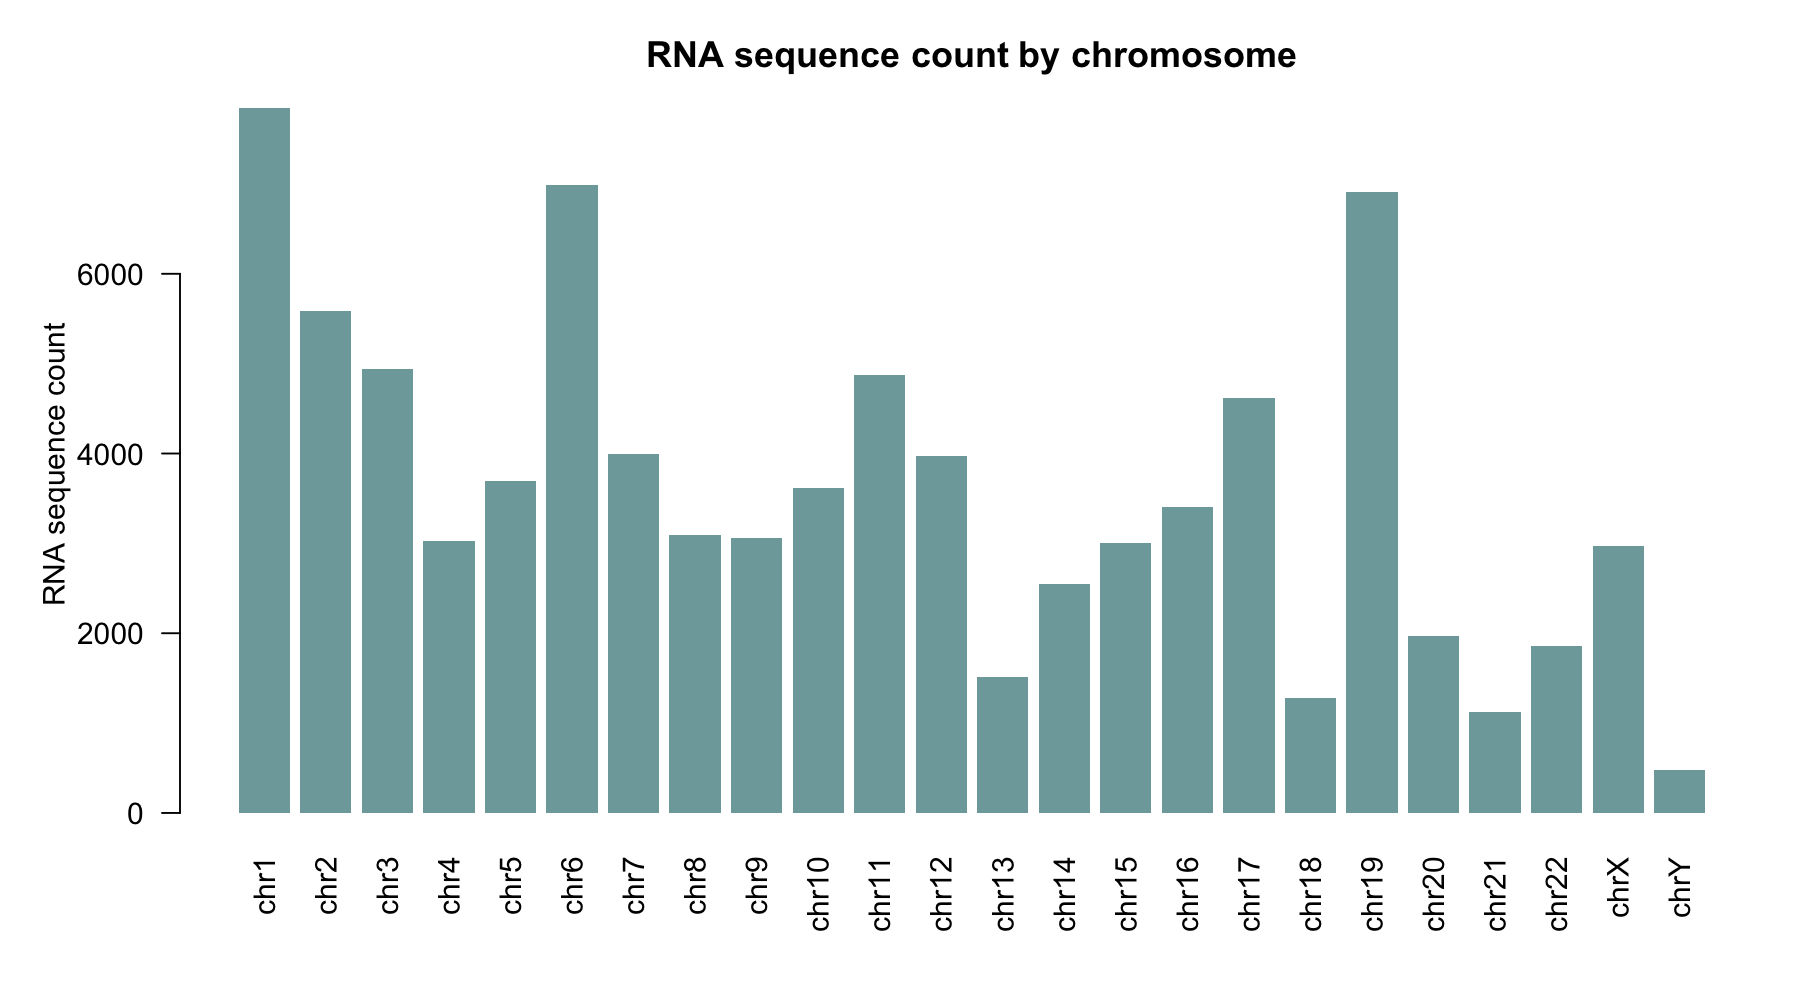
\includegraphics[width=0.92\textwidth]{chr_rna_counts_barplot.png}
\caption{各染色体 RNA 序列数量统计}
\end{figure}

\begin{figure}[H]
\centering
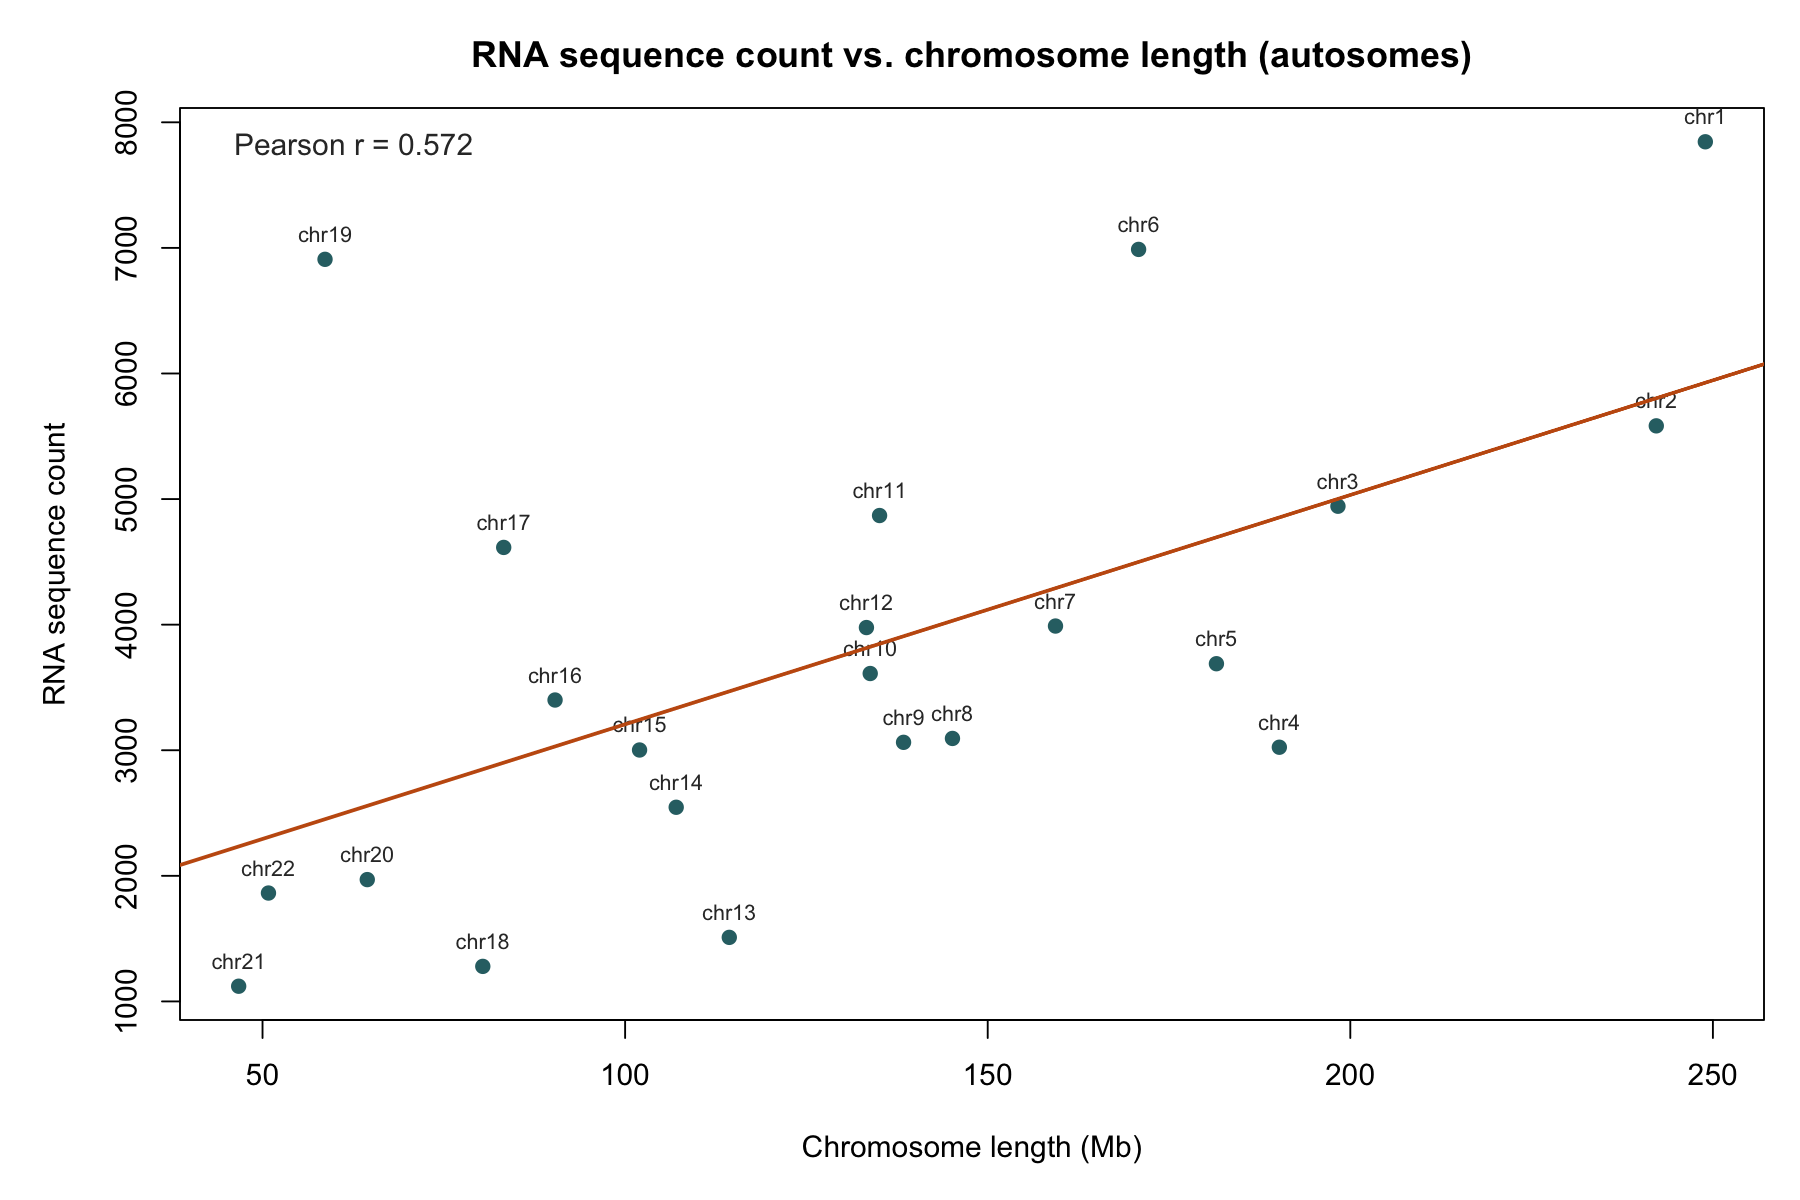
\includegraphics[width=0.92\textwidth]{chr_length_vs_rna_count.png}
\caption{常染色体长度与 RNA 序列数量关系}
\end{figure}

\begin{table}[H]
\centering
\caption{常染色体 RNA 序列数量与染色体长度}
\small
\begin{tabular}{rrrr}
\toprule
染色体 & 长度/Mb & RNA 序列数 & 每 Mb 序列数 \\
\midrule
chr1 & 248.96 & 7845 & 31.51 \\
chr2 & 242.19 & 5583 & 23.05 \\
chr3 & 198.30 & 4943 & 24.93 \\
chr4 & 190.21 & 3024 & 15.90 \\
chr5 & 181.54 & 3689 & 20.32 \\
chr6 & 170.81 & 6988 & 40.91 \\
chr7 & 159.35 & 3989 & 25.03 \\
chr8 & 145.14 & 3094 & 21.32 \\
chr9 & 138.39 & 3063 & 22.13 \\
chr10 & 133.80 & 3611 & 26.99 \\
chr11 & 135.09 & 4869 & 36.04 \\
chr12 & 133.28 & 3977 & 29.84 \\
chr13 & 114.36 & 1510 & 13.20 \\
chr14 & 107.04 & 2546 & 23.78 \\
chr15 & 101.99 & 3002 & 29.43 \\
chr16 & 90.34 & 3400 & 37.64 \\
chr17 & 83.26 & 4615 & 55.43 \\
chr18 & 80.37 & 1279 & 15.91 \\
chr19 & 58.62 & 6909 & 117.87 \\
chr20 & 64.44 & 1970 & 30.57 \\
chr21 & 46.71 & 1121 & 24.00 \\
chr22 & 50.82 & 1863 & 36.66 \\
\bottomrule
\end{tabular}
\end{table}

常染色体长度与 RNA 序列数量存在中等正相关，但并不严格成比例。如果二者严格成比例，散点图中的点应大致沿一条直线分布；实际结果中 chr19 长度较短却有较高 RNA 序列数，而 chr13、chr18 等染色体的 RNA 序列数量相对较低。这说明染色体 DNA 长度不能单独解释 RNA 序列数量。

可能影响该关系的因素包括可变剪接产生的多个转录本、非编码 RNA 注释数量、重复序列和异染色质比例、参考注释数据库的收录标准，以及替代单倍型或未放置序列是否被纳入统计。因此，本实验中的 RNA 序列数量更接近转录本注释密度的结果，而不是简单由染色体长度决定。

\section{讨论}

\subsection{Linux 在生物信息学任务中的优势}

Linux 的一个重要特点是命令行工具丰富、文本处理能力强，并且不同命令之间可以通过管道和重定向连接起来。这种特点很适合生物信息学中常见的文件筛选、格式转换、批量统计和流程化分析。例如本实验中，\texttt{grep} 可以直接从 FASTA 文件中筛选特定染色体，\texttt{wc} 可以统计行数，\texttt{>} 可以把结果保存到新文件，Bash 脚本又可以把这些命令组织成可重复运行的流程。

Linux 还具有稳定、轻量、便于远程运行和便于自动化的优势。很多生物信息学软件最先支持或主要支持 Linux 环境，尤其是涉及基因组注释、序列比对、变异检测、转录组分析和大规模文件处理的软件。对于需要处理大量样本、文件体积很大、步骤重复性强、需要在服务器或高性能计算平台运行的问题，Linux 往往比图形界面软件更合适。

具体来说，Linux 最适合以下类型的问题：第一，大规模文本型数据处理，例如 FASTA、FASTQ、VCF、GTF、BED 等文件的筛选和统计；第二，需要批量重复运行的分析，例如对多个样本循环进行质控、比对和计数；第三，需要组合多个软件形成分析流程的问题，例如从原始测序数据到差异表达分析的 pipeline；第四，需要在远程服务器、集群或云平台运行的任务。相对而言，如果任务只是少量数据的手动浏览或简单绘图，图形界面工具可能更直观；但一旦涉及可重复性和规模化，Linux 的优势就会更加明显。

\subsection{不同染色体 RNA 密度与染色体功能的关系}

本实验用每 Mb RNA 序列数量近似表示 RNA 密度。结果显示，不同染色体之间 RNA 密度差异很大，这种差异并不只是由染色体长度决定，也可能与转录本注释策略、可变剪接复杂度、非编码 RNA 收录情况和染色体功能区域组成有关。下面选取三个比较特别或反常的染色体进行讨论。

首先，chr19 是最突出的例子。chr19 的长度只有约 58.62 Mb，但 RNA 序列数达到 6909，每 Mb RNA 序列数约为 117.87，是本实验中密度最高的常染色体之一。这说明 chr19 虽然短，但 RefGene 中记录的转录本非常密集。chr19 上存在与免疫、锌指蛋白、信号调控和代谢相关的基因簇，这些区域可能带来较多转录本注释和剪接异构体，因此它的 RNA 注释密度明显高于许多更长的染色体。

其次，chr17 也是一个相对反常的例子。chr17 长度约 83.26 Mb，并不属于最长的染色体，但 RNA 序列数为 4615，每 Mb RNA 序列数约为 55.43，明显高于多数常染色体。chr17 上有较多与细胞周期、DNA 修复、发育调控和疾病相关的基因，例如一些肿瘤研究中常见的重要基因也位于 chr17。因此，chr17 的高 RNA 密度可能反映了其较高的基因和转录本注释密度。

第三，chr13 和 chr18 是相反方向的例子。chr13 长度约 114.36 Mb，但 RNA 序列数只有 1510，每 Mb RNA 序列数约为 13.20；chr18 长度约 80.37 Mb，RNA 序列数为 1279，每 Mb RNA 序列数约为 15.91。这两个染色体并不算特别短，但 RNA 密度较低，说明其在 RefGene mRNA 文件中收录的转录本数量相对较少，也可能与较多重复、异染色质相关区域或较低的转录本注释复杂度有关。与 chr19 和 chr17 相比，它们提示染色体长度较大并不必然对应更多 RNA 序列。

因此，不同染色体上的 RNA 密度可能与染色体功能存在一定关联，但这种关联并不是简单的一一对应关系。更准确地说，本实验中的 RNA 密度首先是 RefGene 转录本注释密度的结果，它可能受到转录本冗余、注释策略、功能基因簇分布、染色质开放程度和选择压力等因素共同影响。

\subsection{RNA 密度影响因素假设的验证方式}

本实验提出的一个主要假设是：不同染色体 RNA 密度差异可能由转录本注释策略、可变剪接复杂度、非编码 RNA 注释数量、染色质状态、表达证据和参考数据库完整度共同决定。要验证这些假设，可以从多个层面进一步分析。

第一，可以验证本实验结果是否受注释数据库影响。因为这里统计的是 RefGene mRNA FASTA 中的描述行，不同数据库对转录本的收录标准并不完全相同。可以分别使用 RefGene、Ensembl 和 GENCODE 重新统计每条染色体的转录本数量，并比较 chr19、chr17、chr13 和 chr18 等染色体的排序是否稳定。如果不同数据库下结果差异很大，说明本实验中的 RNA 密度更接近“数据库注释密度”，而不能直接解释为染色体真实转录活跃程度。

第二，可以验证可变剪接和转录本冗余是否影响 RNA 密度。因为本实验统计的是序列描述行，同一个基因可能对应多个转录本。如果某些染色体上同一基因拥有更多剪接异构体，它们的 RNA 序列数也会偏高。可以把 FASTA 中的转录本进一步映射回基因，计算每条染色体的“转录本数/基因数”，再比较 chr19、chr17、chr13、chr18 等染色体之间是否存在明显差异。

第三，可以验证非编码 RNA 和功能基因簇的影响。可以分别统计每条染色体上的 protein-coding RNA、lncRNA、miRNA、pseudogene 转录本数量，再观察高 RNA 密度染色体是否由某类 RNA 特别富集造成。同时，也可以对高密度染色体上的基因做 GO 或通路富集分析，判断是否富集于免疫、转录调控、代谢或发育等功能类别。

第四，可以从染色质状态和表达证据角度验证。RNA 序列注释数量不等于实际表达量，因此可以进一步结合 GTEx、ENCODE 或 RNA-seq 数据，比较不同染色体上真实表达的基因数、平均表达量和组织特异性。如果某条染色体注释密度高但实际表达较低，说明注释数量和功能活跃程度不能完全等同。

最后，还可以从基因组结构角度验证。可以比较不同染色体的 GC 含量、开放染色质区域比例、CpG island 密度、复制时间和保守元件分布，再观察这些特征与 RNA 注释密度是否相关。这样可以避免把 RNA 密度简单归因于某一个因素，而是从注释、表达和染色质结构三个层面综合判断。

\section{结论}

本实验完成了 Linux 基础文件操作、ANNOVAR 解压与示例文件查看、FASTA 文件筛选、Bash 脚本统计和 R 可视化分析。主要结论如下：

\begin{itemize}
  \item ANNOVAR 已成功解压，并可以查看 example 目录和 humandb FASTA 文件；
  \item FASTA 描述行以 ``>'' 开头，包含转录本编号和染色体位置信息；
  \item \texttt{hg38\_refGeneWithVerMrna.fa} 中 chr21 相关 RNA 序列描述行为 1121 条；
  \item chr1--chr22 的 RNA 序列数量差异明显，chr1、chr6、chr19 数量较高，chr18、chr21 较低；
  \item 常染色体长度与 RNA 序列数量的 Pearson 相关系数为 0.572，说明二者有一定正相关，但并不严格成比例。
\end{itemize}

\section{引用与 AI 使用说明}

\subsection{数据集与软件}

\begin{itemize}
  \item 课程材料：\texttt{c4.Linux\_basics.pdf}。
  \item 分析软件：ANNOVAR。
  \item 输入文件：\texttt{bioinfor/annovar/humandb/hg38\_refGeneWithVerMrna.fa}。
  \item 软件环境：macOS 终端、Bash、R 4.5.2、\LaTeX。
\end{itemize}

\subsection{AI 使用说明}

本实验在课程 PDF 阅读、终端记录整理、结果文件汇总、R 可视化脚本补充和实验报告排版过程中使用了 AI 辅助。AI 的主要用途包括：

\begin{itemize}
  \item 根据课程 PDF 提取实验要求和得分点；
  \item 根据 \texttt{终端保存的输出.txt} 整理已完成的 Linux 命令和结果；
  \item 补充常染色体 RNA 序列统计、相关性分析和可视化；
  \item 按照既往实验报告 PDF 的 LaTeX 风格整理本次实验报告。
\end{itemize}

需要说明的是，所有统计结果、图表和文件均基于本地工作目录中的实际文件生成；最终报告内容经过人工检查和修改。

\subsection{代表性提示词}

\begin{itemize}
  \item 阅读这个文档里的 PDF，了解此次生信实验课程需要的东西，帮我完成并输出一份实验报告。
  \item 期中 txt 文件是我课上已经用终端完成的内容，需要导出的结果应该也在其中的某个文件夹里面，你自行整理一下，我完成的部分可以直接用。
  \item 我希望按照 PDF 里每个地方的得分点都展示出来。
  \item 每一分给我写成一个单独实验结果，包括 Linux 代码和结果。
  \item 按照之前实验报告 PDF 的格式整理，变成 LaTeX 输出 PDF。
\end{itemize}

\end{document}
